Данные были собраны из открытых источников \cite{libmipt}\cite{mathedu}. 

\begin{figure}[h]
    \centering
    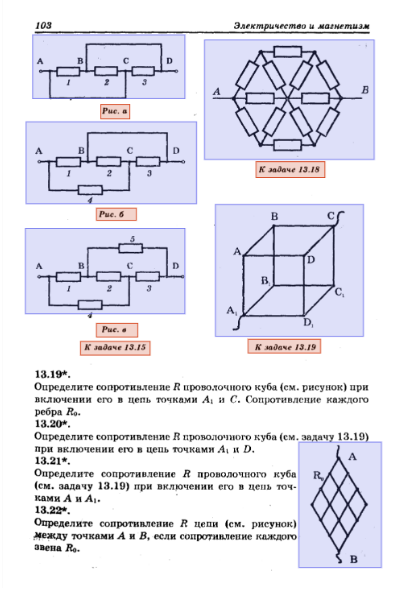
\includegraphics[width=0.5\textwidth]{assets/dataset/kirik_labeling.png}
    \caption{Пример аннотированной иллюстрации из книги Генденштейн, Кирик, Гельфгат: 1001 задача по физике}
    \label{annotation}
\end{figure}



Для получения обучающей выборки была проведена разметка части датасета. Каждое изображение включает в себя текстовую информацию, а также различные чертежи и формулы, характерные для данной области знаний.

Процесс разметки включал создание аннотаций для каждого изображения, а именно выделение границ объектов, таких как текстовые блоки, формулы и чертежи. Этот процесс требовал точности и внимательности для корректного определения границ объектов на изображении и их соответствия с аннотациями.

Для расширения датасета и обеспечения его разнообразия была применена аугментация данных. Применялись повороты, масштабирование, изменение освещения и отражение, позволили создать дополнительные вариации входных данных. 
Это способствовало увеличению разнообразия обучающей выборки и повышению устойчивости модели к различным вариациям данных, что важно для обеспечения ее эффективности в реальных условиях различной разметки страницы.
